%!TEX root = ../thesis.tex
%*******************************************************************************
%****************************** Third Chapter **********************************
%*******************************************************************************
\chapter{High quality assembly of a single Mosquito}

% **************************** Define Graphics Path **************************
\ifpdf
    \graphicspath{{Chapter3/Figs/Raster/}{Chapter3/Figs/PDF/}{Chapter3/Figs/}}
\else
    \graphicspath{{Chapter3/Figs/Vector/}{Chapter3/Figs/}}
\fi



\section{Background}

Exciting efforts to sequence the diversity of life are building momentum \cite{Lewin2018-lc} but one of many challenges that these efforts face is the small size of most organisms. For example, arthropods, which comprise the most diverse animal phylum, are typically small. Beyond this, while levels of heterozygosity within species vary widely across taxa, intraspecific genetic variation is often highest in small organisms \cite{Leffler2012-uh}. Over the past two decades, reference genomes for many small organisms have been built through considerable efforts of inbreeding organisms to reduce their heterozygosity levels such that many individuals can be pooled together for DNA extractions. This approach has varied in its success, for example working well for organisms that are easy to inbreed (e.g., many Drosophila species \cite{Drosophila_12_Genomes_Consortium2007-fx}), but less well for species that are difficult or impossible to inbreed (e.g., Anopheles \cite{Neafsey2015-op}). Therefore, many efforts to sequence genomes of small organisms have relied primarily on short-read approaches due to the large amounts of DNA required for long-read approaches. For example, the recent release of 28 arthropod genomes as part of the i5K initiative used four different insert size Illumina libraries, resulting in an average contig N50 of 15 kb and scaffold N50 of 1 Mb \cite{Thomas2018-rk}.


Another way to overcome DNA input requirements, while also reducing the number of haplotypes present in a DNA pool, is to limit the number of haplotypes in the pool of individuals by using offspring from a single cross. This is easier than multiple generations of inbreeding, and can be successful. For example, a recent PacBio Aedes aegypti assembly used DNA extracted from the offspring of a single cross, thus reducing the maximum number of haplotypes for any given locus to four, thereby improving the assembly process and achieving a contig N50 of 1.3 Mb \cite{Matthews2018-th}.

However, for an initiative like the Earth BioGenome Project \cite{Lewin2018-lc}  that aims to build high-quality reference genomes for more than a million described species over the next decade, generating broods to reach sufficient levels of high molecular weight DNA for long-read sequencing will be infeasible for the vast majority of organisms. Therefore, new methods that overcome the need to pool organisms are needed to support the creation of reference-quality genomes from wild-caught individuals to increase the diversity of life for which reference genomes can be assembled. Here, we present the first high-quality genome assembled with unamplified DNA from a single individual insect using a new workflow that greatly reduces input DNA requirements.

Until recent advances in long read library prep \cite{mosquito_assembly}, it was not possible to obtain
enough DNA from a single individual of small organisms such as mosquitos to create a long-read sequencing library from one individual. 
But for many other smaller species, this remains the case. And it also remains the case for nanopore sequencing. 
Whether it is possible to decrease the input requirements for nanopore sequencing and to what extent are currently unknown.  


\section{DNA Isolation}

The DNA isolation was carried out by Juliana Cudini, a fellow PhD student. 

High molecular weight (HMW) DNA was isolated from a single \textit{Anopheles coluzzii} female from the Ngousso colony. This colony was created in 2006 from the broods of approximately 100 wild-caught pure \textit{Anopheles coluzzii} females in Cameroon (pers. comm. Anna Cohuet). Although the colony has been typically held at >100 breeding individuals, given the long time since colonization, there is undoubtedly inbreeding. A single female was ground in 200 $\mu l$ PBS using a pestle with several up and down strokes (i.e., no twisting), and DNA extraction was carried out using a Qiagen MagAttract HMW kit (PN-67653) following the manufacturer?s instructions, with the following modifications: 200 $\mu l$ 1X PBS was used in lieu of Buffer ATL; PBS was mixed simultaneously with RNAse A, Proteinase K, and Buffer AL prior to tissue homogenisation and incubation; incubation time was shortened to 2 h; solutions were mixed by gently flicking the tube rather than pipetting; and subsequent wash steps were performed for one minute. Any time DNA was transferred, wide-bore tips were used. These modifications were in accordance with recommendations from 10X Genomics HMW protocols that aim to achieve >50 kb molecules. The resulting sample contained ~250 ng of DNA, and we used the FEMTO Pulse (Advanced Analytical, Ankeny, IA, USA) to examine the molecular weight of the resulting DNA. This revealed a relatively sharp band at ~150 kb (Figure S1). The DNA was shipped from the U.K. to California on cold packs, and examined again by running 500 pg on the FEMTO Pulse. While a shift in the molecular weight profile was observed as a result of transport, showing a broader DNA smear with mode of ~40 kb (Figure 1), it was still suitable for library preparation (note that this shifted profile is coincidentally similar to what is observed with the unmodified MagAttract protocol). DNA concentration was determined with a Qubit fluorometer and Qubit dsDNA HS assay kit (Thermo Fisher Scientific, Waltham, MA, USA), and 100 ng from the 250 ng total was used for library preparation.



\begin{figure}[!ht]
\caption{\textit{Anopheles coluzzii} input and resulting library DNA lengths}
\label{figure:fempto}
\begin{centering}
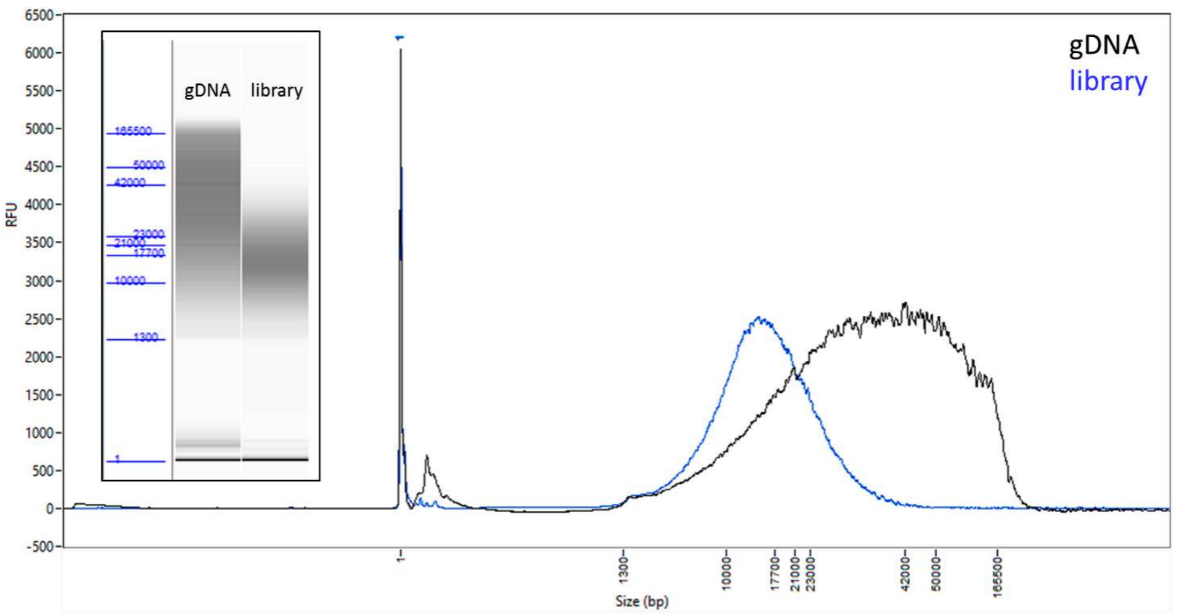
\includegraphics[width=.60\textwidth]{fempto.png}
\subcaption{ FEMTO Pulse traces and ?gel? images (inset) of the genomic DNA input (black) and the final library (blue) before sequencing. }
\end{centering}
\end{figure}

\section{Library prep and Sequencing}

Library prep and sequencing were performed by Sarah Kingan, Senior Scientist at PacBio. 

A SMRTbell library was constructed using an early access version of SMRTbell Express Prep kit v2.0 (Pacific Biosciences, Menlo Park, CA, USA). Because the genomic DNA was already fragmented with the majority of DNA fragments above 20 kb, shearing was not necessary. 100 ng of the genomic DNA was carried into the first enzymatic reaction to remove single-stranded overhangs followed by treatment with repair enzymes to repair any damage that may be present on the DNA backbone. After DNA damage repair, ends of the double stranded fragments were polished and subsequently tailed with an A-overhang. Ligation with T-overhang SMRTbell adapters was performed at 20 C for 60 min. Following ligation, the SMRTbell library was purified with two AMPure PB bead clean up steps (PacBio, Menlo Park, CA), first with 0.45X followed by 0.80X AMPure. The size and concentration of the final library (Figure  \ref{figure:fempto}) were assessed using the FEMTO Pulse and the Qubit Fluorometer and Qubit dsDNA HS reagents Assay kit (Thermo Fisher Scientific, Waltham, MA, USA), respectively.
Sequencing primer v4 and Sequel DNA Polymerase 3.0 were annealed and bound, respectively, to the SMRTbell library. The library was loaded at an on-plate concentration of 5?6 pM using diffusion loading. SMRT sequencing was performed on the Sequel System with Sequel Sequencing Kit 3.0, 1200 min movies with 120 min pre-extension and Software v6.0 (PacBio). A total of 3 SMRT Cells were run.


\section{Assembly}

As previously discussed, recent advances in Pacbio library prep have reduced the DNA input requirement to a level (100ng) at which it is 
possible to create a long read library from a single mosquito. Of course sequencing a single individual is beneficial to assembly over 
sequencing a pool of individuals as the problem that heterozygosity imposes on assembly is greatly exacerbated due to the additional haplotypes 
in a pool of individuals over the two haplotypes contained in a single individual. 

High molecular weight DNA was isolated from a single An. coluzzii female mosquito and shipped to Pacbio for early access low input 
library preparation and sequencing. We obtained three SMRT cells of Pacbio long read data. This data was assembled using the Falcon-Unzip 
software with the median length subread per ZMW for a for a total of 12.8 Gb of sequence which equates to roughly 48x coverage of the expected 
genome size. The resulting primary assembly consisted of 372 contigs totaling 266 Mb in length, with a contig N50 of 3.5 Mb and a secondary 
haplotype assembly totalling 78.5 Mb. \ref{table:assemblydata} shows various assembly statistics of the long read assembly and the current 
reference assembly of the closely related \textit{Anopheles gambiae}\cite{PEST}\cite{PESTupdate}\cite{PESTchromitin}\cite{gambiaeref}. 

\section{Curation}

\section{Assembly statistics}



\begin{table}[h!]
\caption{Assembly statistics}
\label{table:assemblydata}
\begin{center}
\begin{tabular}{ | l | l | l | l | l |}
\hline
\multicolumn{2}{|c|}{} & Pacbio Raw & Pacbio Curated & Sanger Assembly \\
\hline

\multirow{3}{4em}{Primary Assembly}
& Size (Mb) & 266 & 251 & 224 \\
\cline{2-5}
& No. Contigs & 372 & 206 & 27,063 \\
\cline{2-5}
& Contig N50 (Mb) & 3.52	& 3.47	& 0.025 \\
\hline%\cline{2-5}
\multirow{3}{4em}{Alternate Haplotigs}
& Size (Mb) & 78.5 & 	89.2	& unresolved \\
\cline{2-5}
& No. Contigs & 665 &	830& 	N/A \\
\cline{2-5}
& Contig N50 (Mb) & 0.22	& 0.199	& N/A \\
\hline
\end{tabular}
\end{center}
\end{table}
The contigs were screened by the Sanger assembly curation team to identify contaminants and mitochondrial sequence identifying two mitochondrial contigs and one 
complete assembly (4.24 Mb single contig) of \textit{Elizabethkingia anophelis}, which is a common gut microbe in \textit{Anopheles} mosquitoes \cite{kingia}. 

\subsection{Quality assessment}

According to Busco \cite{busco} analysis of the primary assembly, 110 genes were duplicated indicating some resolved heterozygosity (haplotigs) remaining in the primary assembly. 
The presence of duplicated haplotypes in a reference genome can result in erroneously low mapping qualities in resequencing studies and cause problems when scaffolding. 
We used the Purge Haplotigs software \cite{purge} and identified 165 primary contigs totalling 10.6 Mb as likely haplotigs which were then moved to the alternate haplotigs fasta.

There are many problems with the current \textit{Anopheles gambiae} reference including 6302 gaps of Ns in the 
primary chromosome scaffolds ranging from 20 bases to 36 kb and 55 gaps of 10 kb that the AGP (A Golden Path) file on Vectorbase annotates as ``contig'' endings. 
This reference also contains a large bin of unplaced contigs (27.3 Mb excluding Ns) designated as the ``UNKN'' (unknown) chromosome. 
However, it is the previously best characterized \textit{Anopheles} assembly which should be very closely related to the \textit{coluzzii} species so 
we endeavored to make comparisons between them. We aligned the assembly contigs to the reference with minimap2 
and then attempted to assign contigs to chromosomes as well as order and orient them. The new assembly is highly concordant with the reference over the entire 
genome, allowing the placement of the long PacBio contigs into chromosomal contexts (figure \ref{figure:dotplot}). We also showed that the assembly 
correctly expanded long repeats that had been collapsed in the reference (figure \ref{figure:repeat}) and that the assembly resolved an incorrect 
order and orientation of the scaffolding of chromosome X (figure \ref{figure:x_inversion}).

We also found that despite running Purge Haplotigs, there remained some haplotig sequence at the ends of contigs (figure \ref{figure:haplotig}) due to the fact that Purge Haplotigs only 
looks for full contigs that have evidence of being a haplotig.



\begin{figure}[!ht]
\section{Comparison to \textit{Anopheles gambiae} PEST reference}
\caption{Comparison of the assembly with the PEST reference}
\label{figure:dotplot}
\begin{centering}
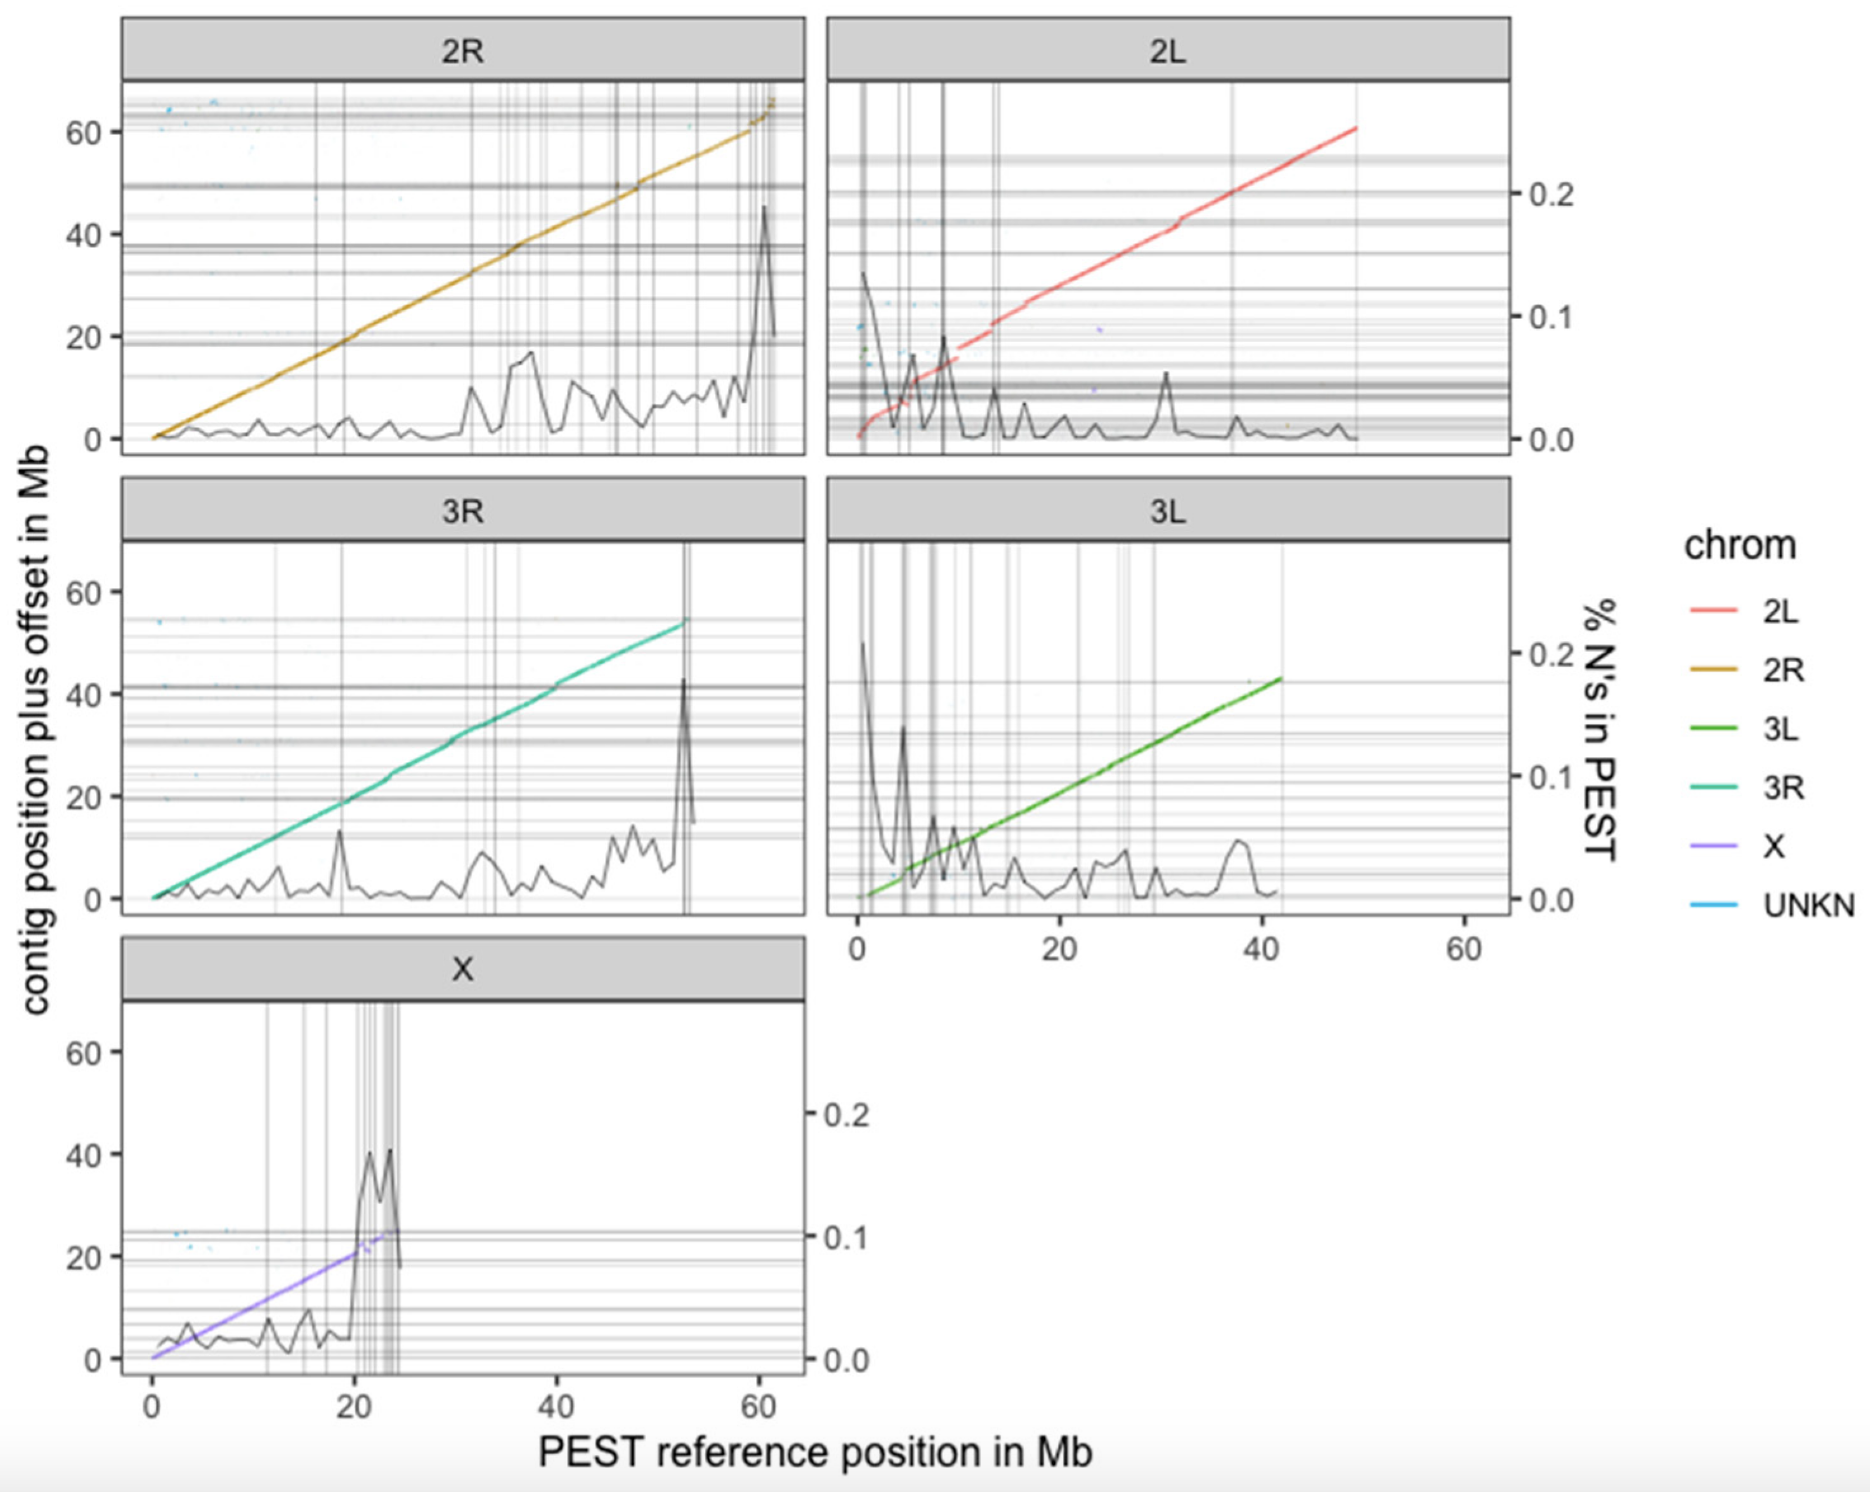
\includegraphics[width=1.0\textwidth]{dotplot.png}
\subcaption{Alignment of the curated PacBio contigs to the AgamP4 PEST reference [21]. Alignments are colored by the primary PEST reference chromosome to which they align but are placed in the panel and Y offset to which the contig as a whole aligns best. Contig ends are denoted by horizontal lines in the assembly and vertical lines in PEST. However, there are many Ns in PEST not annotated as contig breaks so the percent Ns per megabase of PEST is overlaid (scale on the right Y axis). There are no Ns in the PacBio assembly.}
\end{centering}
\end{figure}



\begin{figure}[!ht]
\subsection{Expansion of previously collapsed repeat}
\caption{Example of expansion of previously collapsed repeat}
\label{figure:repeat}
\begin{centering}
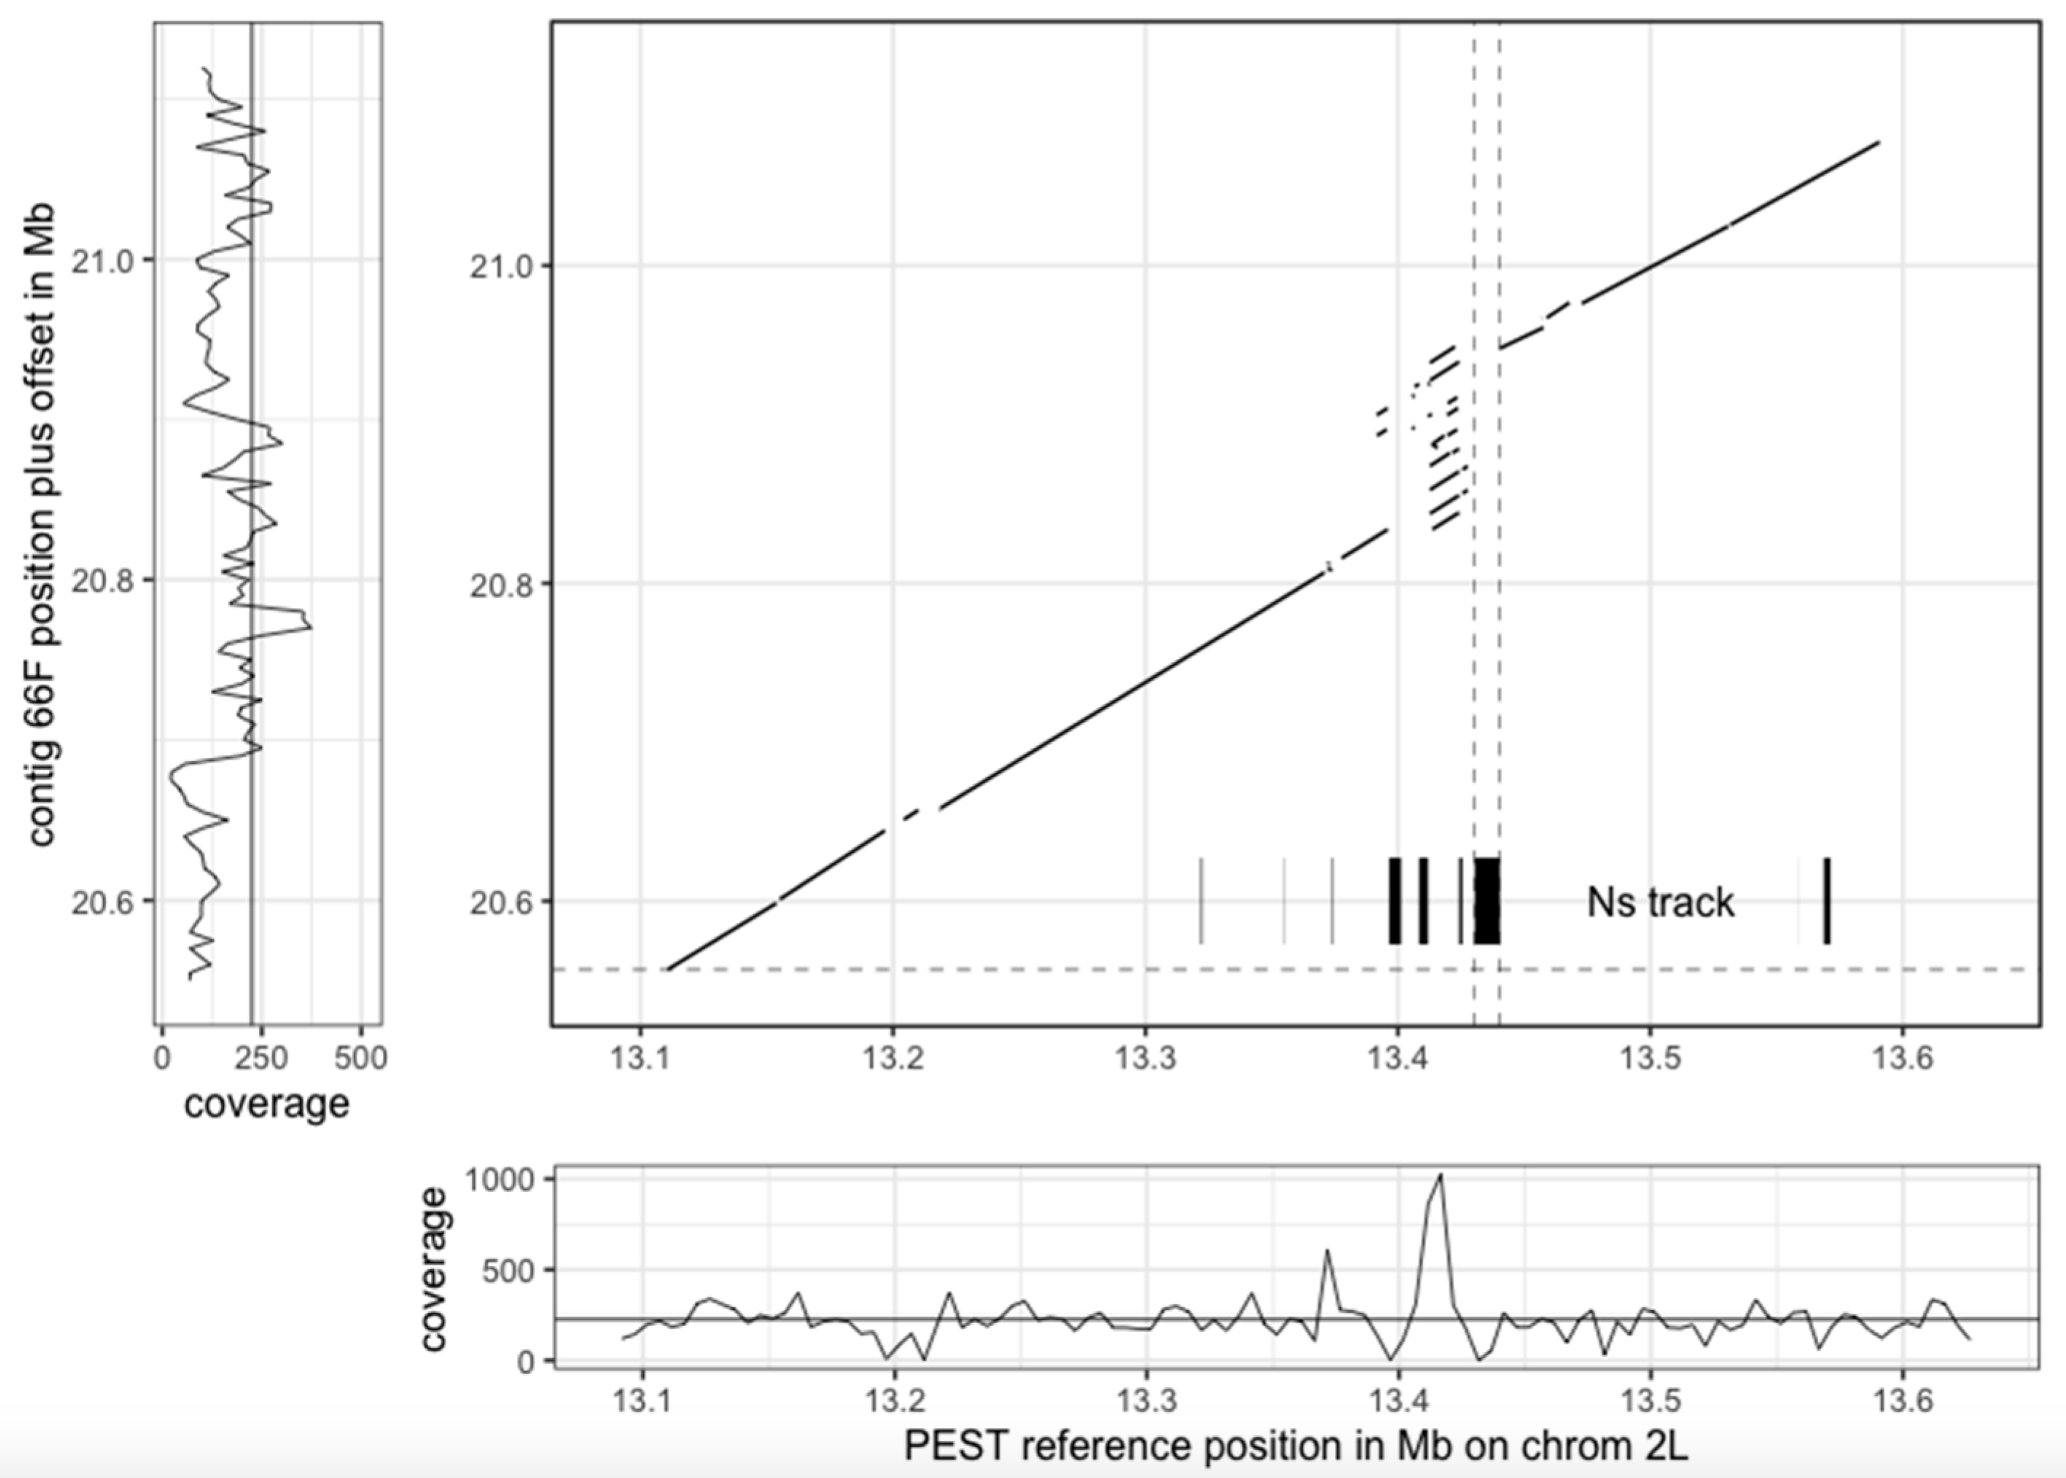
\includegraphics[width=1.0\textwidth]{repeatexpansion.png}
\subcaption{ Example of a compressed repeat in PEST that has been expanded by the PacBio assembly. Dotted vertical lines represent a gap in the PEST assembly (10,000 Ns) between scaffolds, which is now spanned by the single PacBio contig. Coverage plot of the PacBio subreads aligned to PEST (bottom) highlights the region where excess coverage indicates a collapsed repeat in PEST, in contrast the coverage of PacBio subreads aligned to the PacBio contig (left) is more uniform. }
\end{centering}
\end{figure}



\begin{figure}[h!]
\subsection{Corrected order and orientation vs PEST scaffolding}
\caption{Resolved order and orientation error in PEST scaffolding}
\label{figure:x_inversion}
\begin{centering}
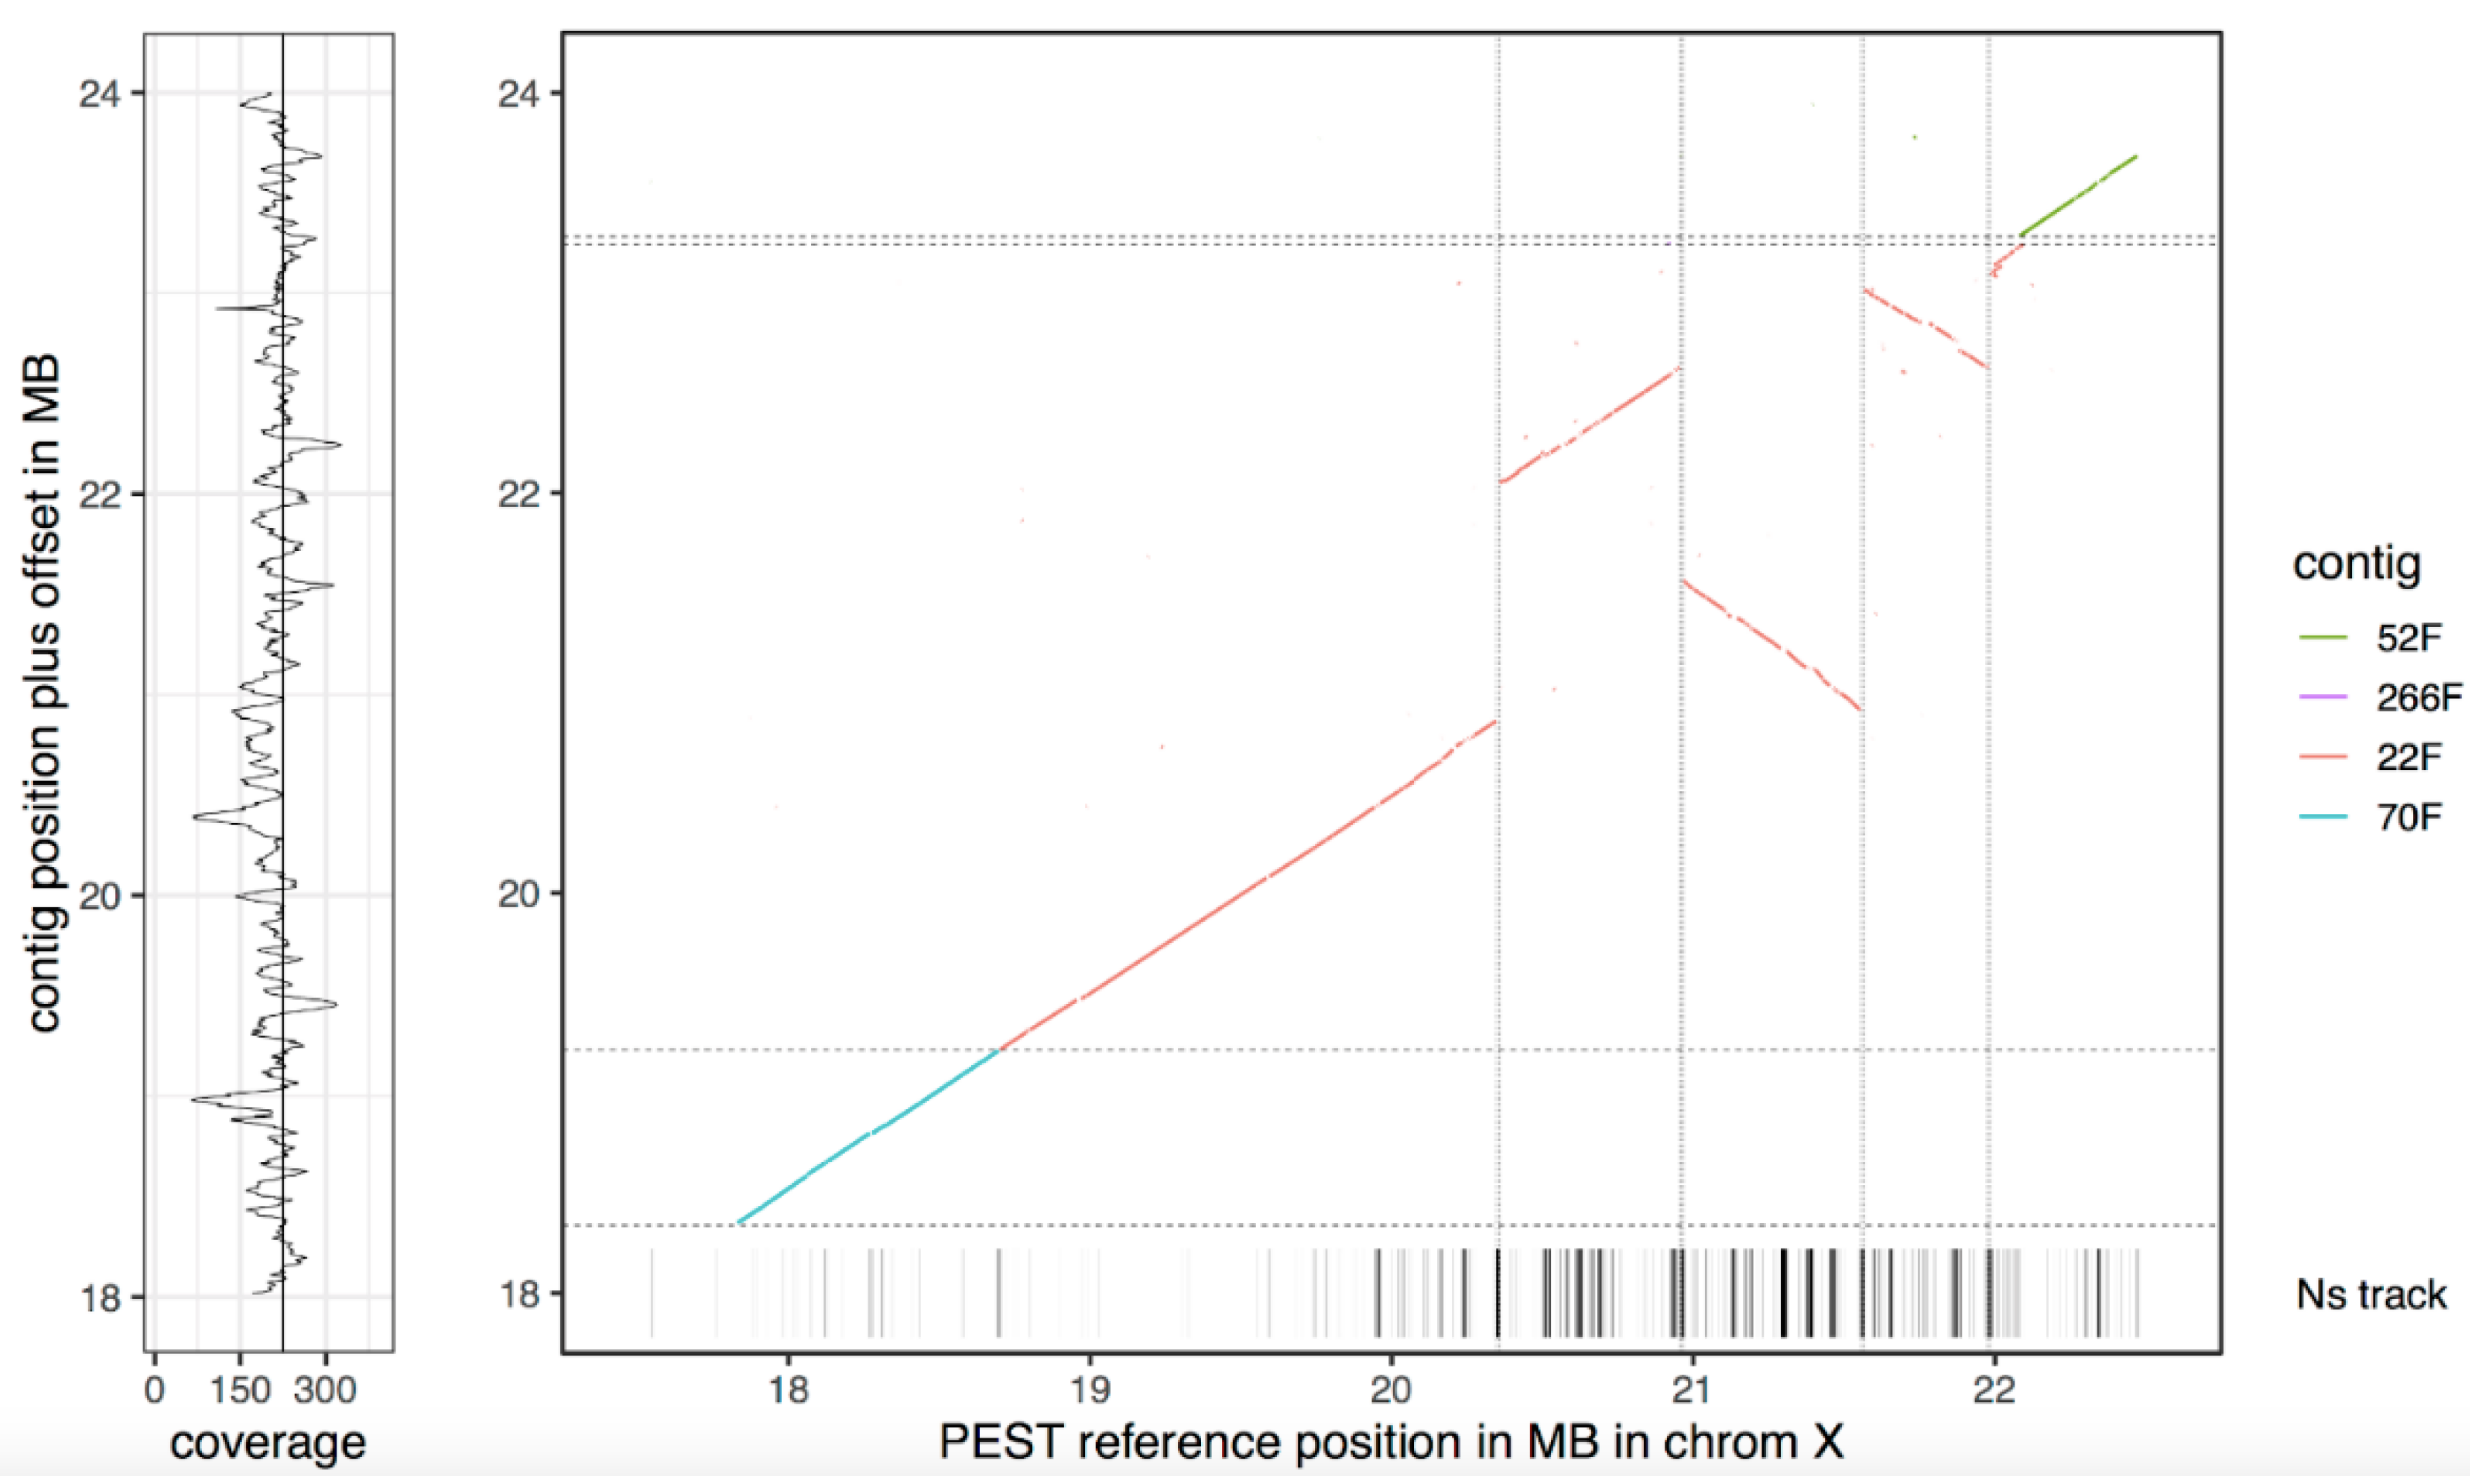
\includegraphics[width=1.0\textwidth]{x_inversion.png}
\subcaption{Alignment of X pericentromeric contigs to PEST, highlighting likely order and orientation issues in the PEST assembly that are resolved by a single PacBio contig.}
\end{centering}
\end{figure}

\begin{figure}[!ht]
\subsection{Identification and correction of misassembly}
\caption{Chimeric assembly}
\label{figure:misassembly}
\begin{centering}
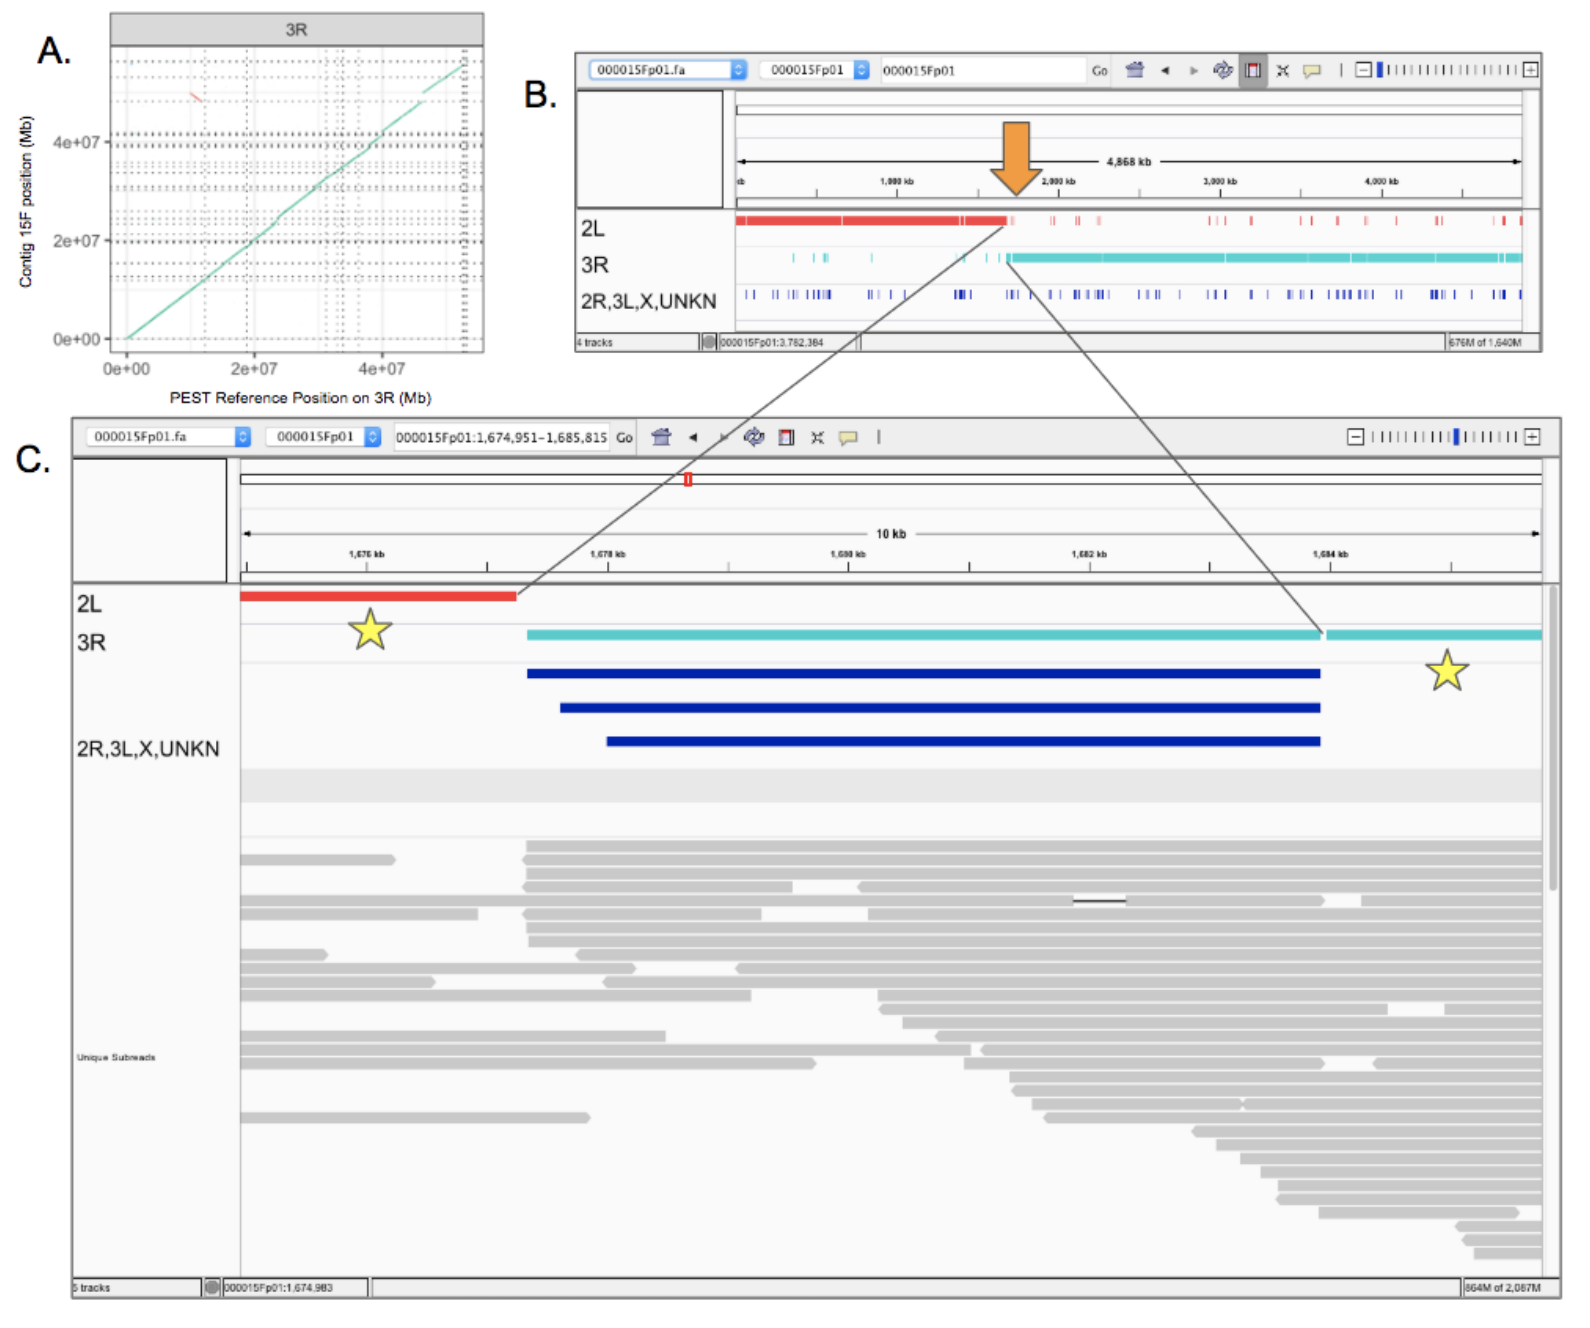
\includegraphics[width=1.0\textwidth]{misassembly.png}
\subcaption{A chimeric contig between 2L and 3R. A. Alignment of PacBio contigs to PEST identifies a candidate chromosomal rearrangement. B. IGV screenshot of breakpoint (orange arrow) localized by alignment of contig to PEST. Red: alignment to 2L, turquoise: alignments to 3R, navy blue: alignments to other chromosomes and unplaced contigs. C. IGV visualization of mapped unique subreads at breakpoint shows 0 subreads mapping across the central repetitive region into the unique flanking sequence on the left (2L) and right (3R) (stars). A count of spanning reads was also determined with bedtools bamtobed utility. The 6.5kb central region aligns to four loci in the PEST genome and has ~370 bp of sequence similarity to the Tc1-like transposase gene in \textit{Anopheles gambiae}.}
\end{centering}
\end{figure}



\begin{figure}[h!]
\subsection{Remaining haplotig sequence on ends of contigs}
\caption{Evidence of remaining haplotig contig ends.}
\label{figure:haplotig}
\begin{centering}
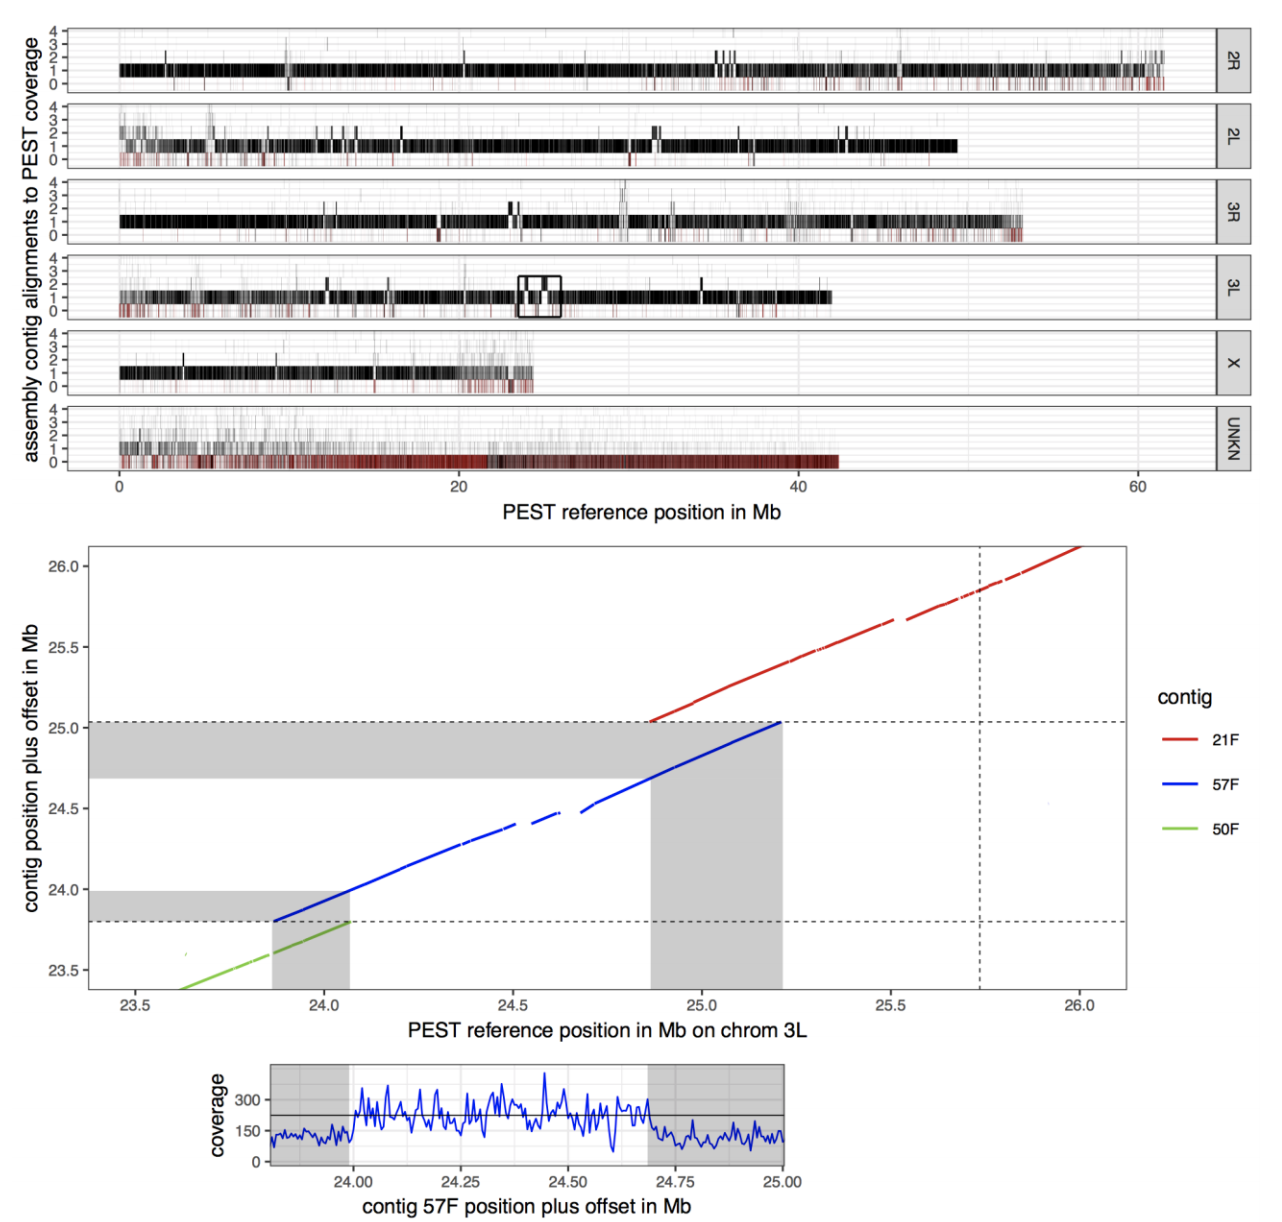
\includegraphics[width=\textwidth]{haplotigity.png}
\subcaption{Alignment and coverage plot (top) of the PacBio assembly contigs relative to PEST,
and magnification of one area of excess coverage (bottom). In the top panel, the number of
alignments of PacBio contigs to PEST are represented by black bars, with most of the genome
showing a 1:1 correspondence to PEST. Red denotes N?s in the reference. Isolated areas of
higher number of contig alignments are visible, one of which (black box) is magnified in the
bottom panel. Here, the ends of neighboring contigs overlap, which is currently not resolved with
the Purge Haplotigs software since the overlap is only partial. The sequencing depth of PacBio
reads for the central (blue) contig (57F) corroborate this interpretation, exhibiting half of the
expected coverage in the greyed regions of contig overlap, and with the corresponding ends of
the red and green contigs complementing with the other half of coverage, respectively (not
shown for clarity).}
\end{centering}
\end{figure}

The PEST annotation also retains a large bin of unplaced contigs (27.3 Mb excluding Ns) designated as the ?UNKN? (unknown) chromosome. We compared the alignments of contigs from the PEST chromosomes (X, 2, 3) versus the contigs from the UNKN to the new assembly. Any regions with a mapping quality score (mapq) 60 alignments of both UNKN and chromosomal contigs are likely to be haplotigs in the UNKN. In total, we find that 7.27 Mb are haplotigs (i.e., also have PEST chromosomal alignments to the same location in the assembly) and another 10.9 Mb are newly placed sequence that do not overlap with PEST chromosomal alignments. The UNKN bin also contains 737 annotated genes. Remarkably, our single-insect assembly now places 667 (>90\%) of these formerly unplaced genes into their appropriate chromosomal contexts (2L:148 genes; 2R:162 genes; 3L: 126 genes; 3R:91 genes; X:140 genes; unplaced:70 genes; details on specific genes can be found in Table S4), which together with their flanking sequence comprise 8.9 Mb of sequence. Altogether, this means that 40\% of the UNKN chromosome is now placed in the genome, along with 90\% of the genes that were contained within it.

\begin{table}[!ht]
\subsection{Placement of previously unplaced genes}
\label{table:unplaced}
\begin{tabular}{ | l | l |}
\hline
 Chromosome arm & Number of placed genes  \\
 
 \hline
 2L & 148 \\
 \hline
 2R & 162 \\
 \hline
 3L & 126 \\
 \hline
 3R & 91 \\
 \hline
 X & 140 \\
 \hline
 unplaced & 70 \\
 \hline
\end{tabular} 
\end{table}




